%-------------------------
% Resume in Latex
% Author : Sourabh Bajaj
% License : MIT
%------------------------

\documentclass[letterpaper,11pt]{article}

\usepackage{latexsym}
\usepackage[empty]{fullpage}
\usepackage{titlesec}
\usepackage{marvosym}
\usepackage[usenames,dvipsnames]{color}
\usepackage{verbatim}
\usepackage{enumitem}
\usepackage[pdftex]{hyperref}
\usepackage{fancyhdr}
\usepackage{graphicx}

\pagestyle{fancy}
\fancyhf{} % clear all header and footer fields
\fancyfoot{}
\renewcommand{\headrulewidth}{0pt}
\renewcommand{\footrulewidth}{0pt}

% Adjust margins
\addtolength{\oddsidemargin}{-0.375in}
\addtolength{\evensidemargin}{-0.375in}
\addtolength{\textwidth}{1in}
\addtolength{\topmargin}{-.5in}
\addtolength{\textheight}{1.0in}

\urlstyle{same}

\raggedbottom
\raggedright
\setlength{\tabcolsep}{0in}

% Sections formatting
\titleformat{\section}{
  \vspace{-4pt}\bfseries
}{}{0em}{}[\color{black}\titlerule \vspace{-5pt}]

%-------------------------
% Custom commands
\newcommand{\resumeItem}[2]{
  \item\small{
    \textbf{#1}{: #2 \vspace{-2pt}}
  }
}

\newcommand{\resumeSubheading}[4]{
  \vspace{-1pt}\item
    \begin{tabular*}{0.97\textwidth}{l@{\extracolsep{\fill}}r}
      \textbf{\small#1} & #2 \\
      \textit{\small#3} & {\small #4} \\
    \end{tabular*}\vspace{-5pt}
}

\newcommand{\resumeSubItem}[2]{\resumeItem{#1}{#2}\vspace{-4pt}}

\renewcommand{\labelitemii}{$\circ$}

\newcommand{\resumeSubHeadingListStart}{\begin{itemize}[leftmargin=*]}
\newcommand{\resumeSubHeadingListEnd}{\end{itemize}}
\newcommand{\resumeItemListStart}{\begin{itemize}}
\newcommand{\resumeItemListEnd}{\end{itemize}\vspace{-5pt}}

%-------------------------------------------
%%%%%%  CV STARTS HERE  %%%%%%%%%%%%%%%%%%%%%%%%%%%%


\begin{document}

%----------HEADING---------------------
\begin{tabular*}{\textwidth}{l@{\extracolsep{\fill}}r}
  \textbf{\Large Jan Michael Laranjo} &  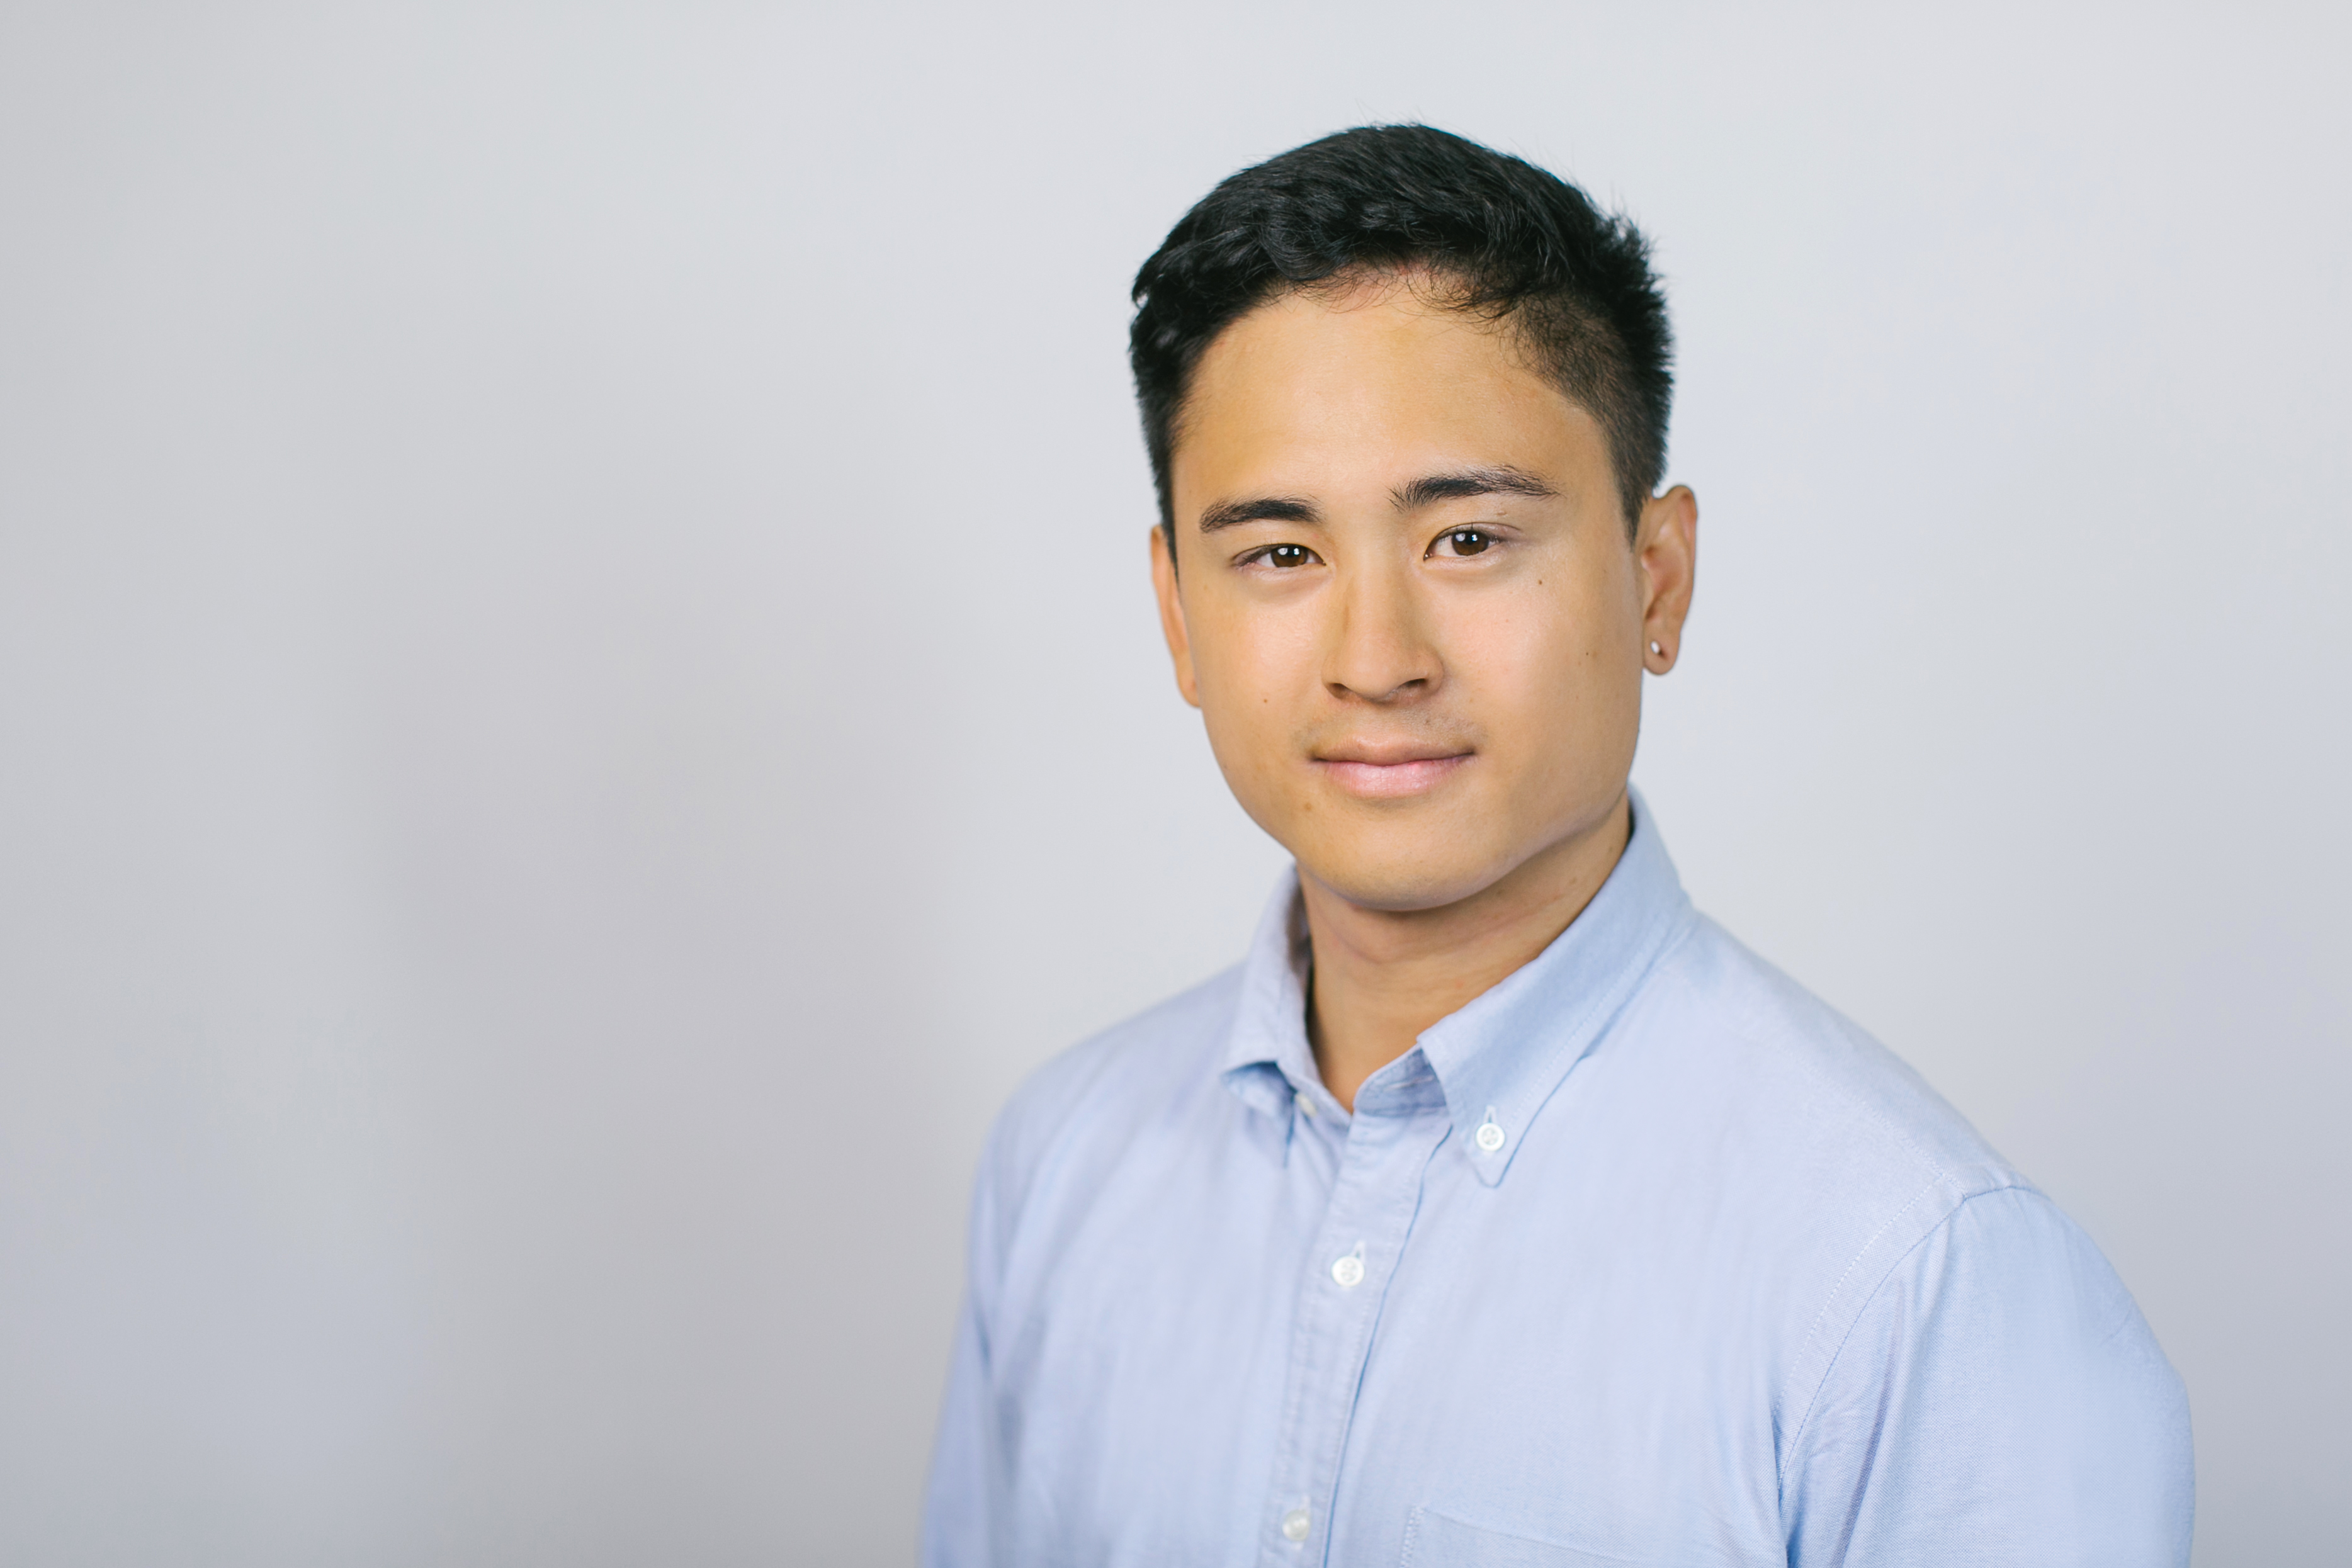
\includegraphics[scale=0.125]{jan.jpg} \\ & Email : \href{mailto:janmichaellaranjo@gmail.com}{janmichaellaranjo@gmail.com}\\
  \href{http://janlaranjo.github.io/}{http://janlaranjo.github.io} & Mobile : +49 676 425 1158\\
  \href{http://https://github.com/janlaranjo/}{https://github.com/janlaranjo} & Barnabitengasse 9/19, 1060 Wien
\end{tabular*}

%-----------AUSBILDUNG----------------
\section{Ausbildung}
  \resumeSubHeadingListStart
	\resumeSubheading
      	{Technische Universit\"at Wien}{Wien}
      	{Bachelorstudium Medieninformatik und Visual Computing}{10/2014 -- dato}
		\begin{itemize}[itemsep=0pt] 
			\item Schwerpunkte in Algorithmen, Datenstrukturen, Softwareentwicklung, Projektmanagement, Qualitätssicherung, Computergraphik, Computer Vision
      \resumeItemListEnd
      
	\resumeSubheading
      	{HTBLuVA Wien 5 Spengergasse}{Wien}
      	{Medieninformatik}{09/2007 – 06/2012}
      	\begin{itemize}[itemsep=0pt] 
			\item Fokus auf Programmieren, Projektmanagement
		\resumeItemListEnd
  \resumeSubHeadingListEnd
%-----------ZERTIFIKATE------------- 
%-----------ERFAHRUNG--------------
\section{Praktische Erfahrung}
  \resumeSubHeadingListStart
    \resumeSubheading
      {MHE \& Partner GmbH}{Wien}
      {Java Developer}{12/2015 – 01/2019}
      \begin{itemize}[itemsep=0pt] 
      	\item Gestaltung und Entwicklung einer UI zum Exportieren von Metadaten aus einem kundeninternen Datawarehouse in ein kundeninternes Format (Java, SQL) 
		\item Entwicklung eines UI-Prototypens für die Benachrichtigung von Mitarbeitern in anderen Abteilungen, um den Arbeitsprozess zu verbessern (Java, SQL, HTML)
		\item Erstellung von Unit-Tests für ein kundeninternes Datawarehouse (Java, JUnit, Mockito, SQL)
		\item Erstellung von automatischen Reports zum Prüfen von fehlenden oder falschen Merkmalen in hausinternen Datenbestände (Java, SQL)
	\resumeItemListEnd

    \resumeSubheading
	{LBC Express}{Manila}
	{Praktikant}{07/2011 – 08/2011}
	\begin{itemize}[itemsep=0pt] 
      	\item IT-Support 
      	\item Aufbau und Wechseln von Peripheriegeräte 
	\resumeItemListEnd
   \resumeSubHeadingListEnd
%-----------ZERTIFIKATE------------- 
%-----------SKILLS----------------------
\section{Skills}
   \resumeSubHeadingListStart
    \resumeSubItem{Sprachen}
      {Java, C++, SQL, Matlab}
    \resumeSubItem{Frameworks}
      {Spring, Hibernate}
    \resumeSubItem{Entwicklungswerkzeuge}
      {Eclipse, IntelliJ, Android Studio, Git, SVN,}
  \resumeSubHeadingListEnd
 
%-----------PROJEKTE------------------ 
  
%-----------ZERTIFIKATE--------------
\section{Zertifikate}
	\begin{itemize}[itemsep=0pt] 
      	\item Oracle Certified Associate, Java SE 8 Programmer
  \resumeSubHeadingListEnd


%-------------------------------------------
\end{document}
